\documentclass[12pt,a4paper,oneside]{ctexart}
\title{\textbf{Practice3 Report}}
\author{22320607 Xu Ziyang}
\date{2023/10/14 YY/MM/DD}
\usepackage{graphicx}
\usepackage{float}
\usepackage{color}
\ctexset{abstractname = {Quick View}}
\ctexset{contentsname = {Contents}}
\begin{document}
    \maketitle
\begin{abstract}
    In today's Report,I will show following things by order:

    1.Code that can change the question to solve displaced by picture.

    2.Model that universal for question 1, 2, 3.

    3.Graph and calculation corresponding to questions and $\omega$.

    (I'm tired of using OpenDocument.Hope \LaTeX \space can make my format better.)
\end{abstract}
\newpage
\tableofcontents 
\newpage
\section{Code}
    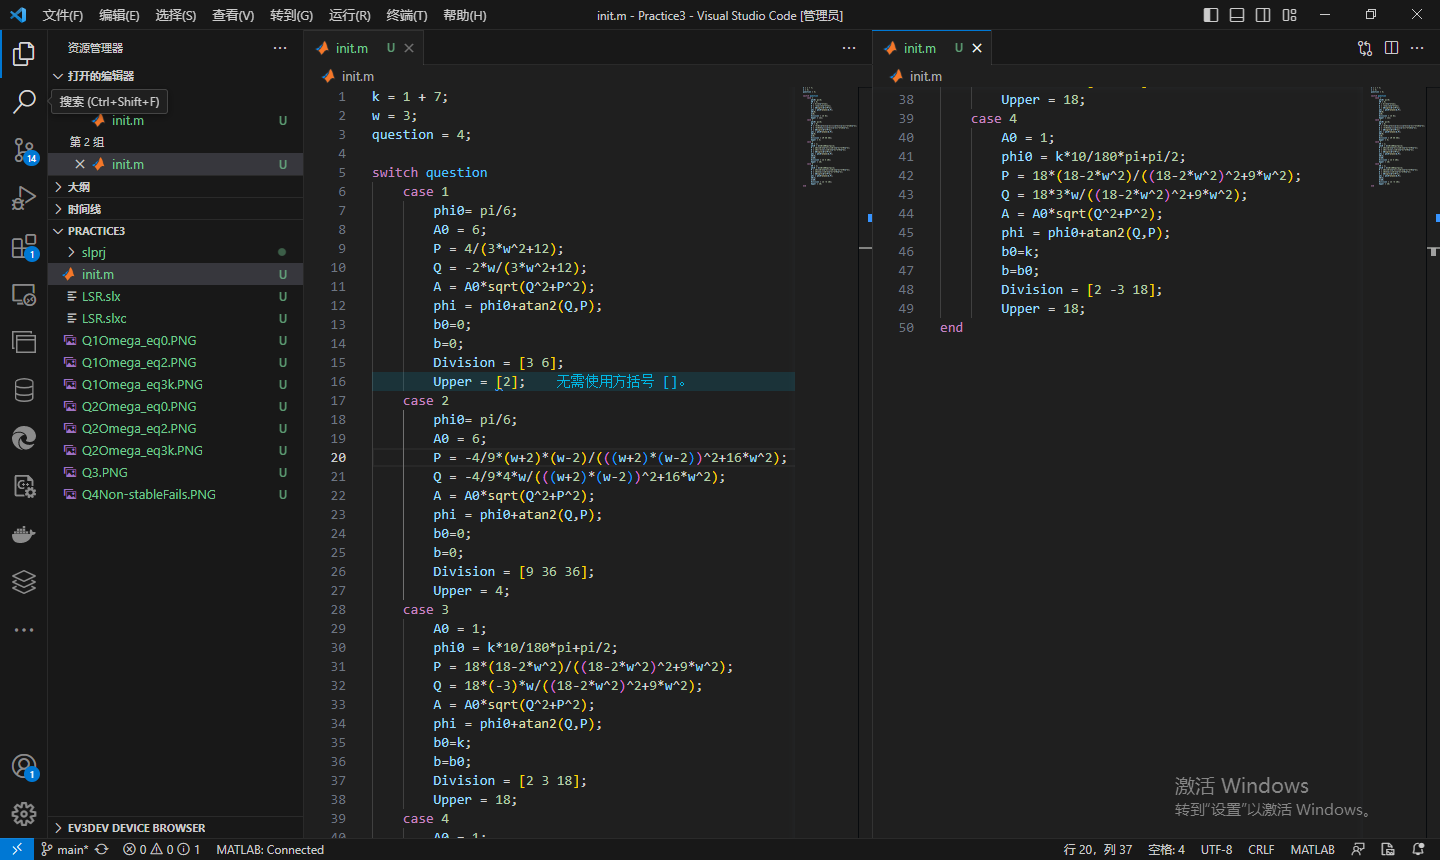
\includegraphics[width = 0.9\linewidth]{Code}

\newpage
\section{Model}
    \subsection*{Main}
        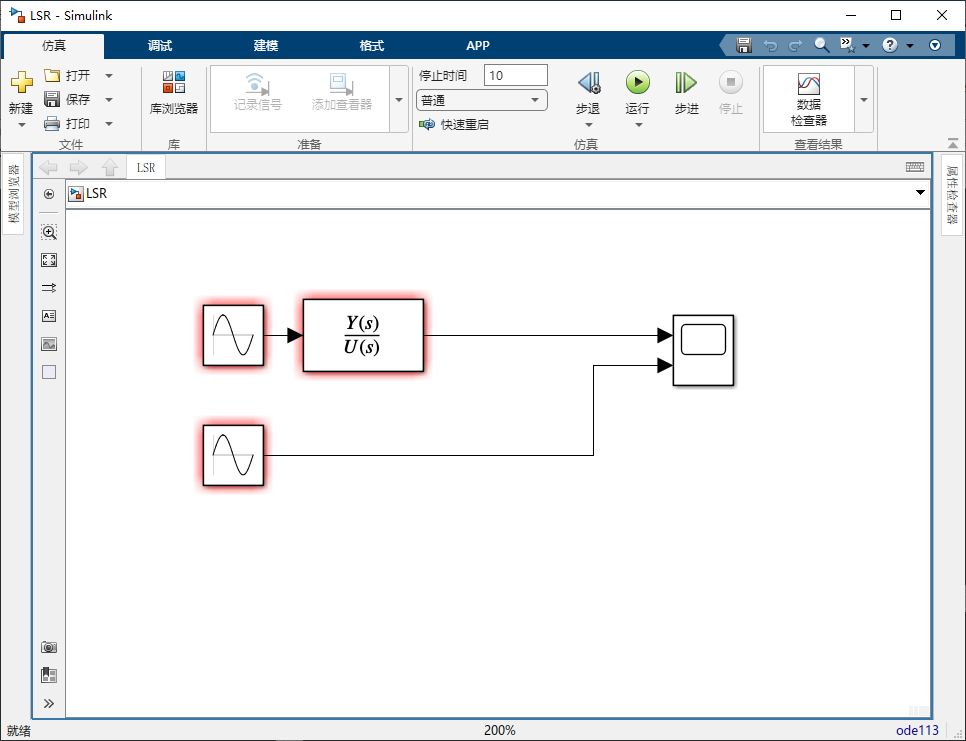
\includegraphics[width = 0.9\linewidth]{Model}
    \subsection*{Detail}
        \textbf{Here are more information of each model and shows which variable is used.}

        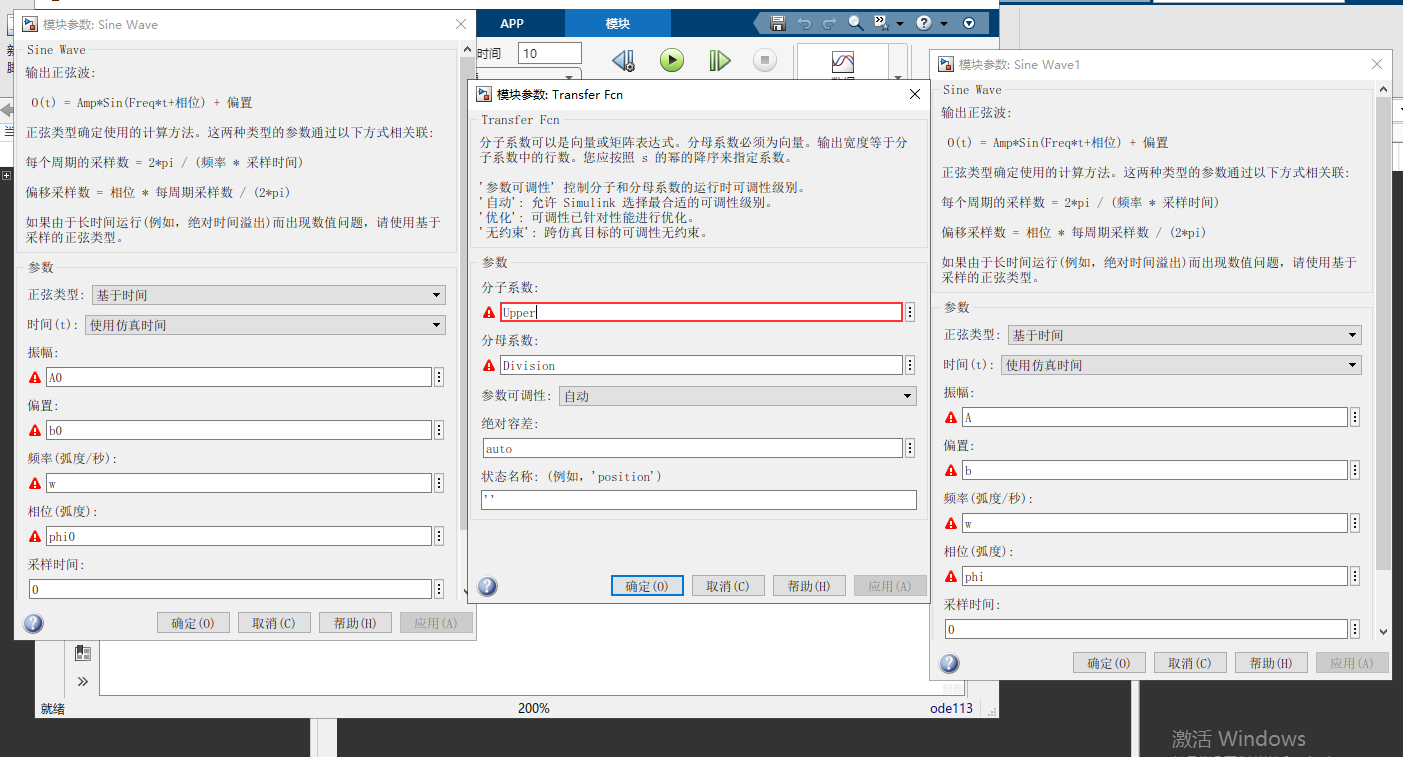
\includegraphics[width = 0.9\linewidth]{Model2.PNG}

\newpage      
\section{Answers}
    \subsection{Question1}
        \subsubsection{Calculation}
            $$3\dot{y}(t) + 6y(t) = 2u(t)$$
            Do laplace transform get:
            $$y(s) = \frac{2}{3s+6}u(s)$$
            $$W(s) = \frac{2}{3s+6}$$
            Let $s = j\omega$.
            $$W(j\omega) = \frac{2}{3j\omega+6}$$
            $$W(j\omega) = \frac{2(6-3j\omega)}{36+9\omega^2}$$
            $$P(\omega) = Re(W(j\omega)) = \frac{12}{36+9\omega^2}$$
            $$Q(\omega) = Im(W(j\omega)) = \frac{-6\omega}{36+9\omega^2}$$
            $$A(\omega) = \sqrt[2]{P(\omega)^2 + Q(\omega)^2} = \frac{\sqrt[2]{144+36\omega^2}}{36+9\omega^2}$$
            $$\phi(\omega) = atan2(Q(\omega),P(\omega))$$
            If $u(t) = Asin(\omega t+\phi_0)+b_0$

            $$y(t) = A(\omega)A_0sin(\omega t + \phi_0 + \phi(\omega)) + b_0$$
        \subsubsection{Graph}
            \begin{figure}[H]
                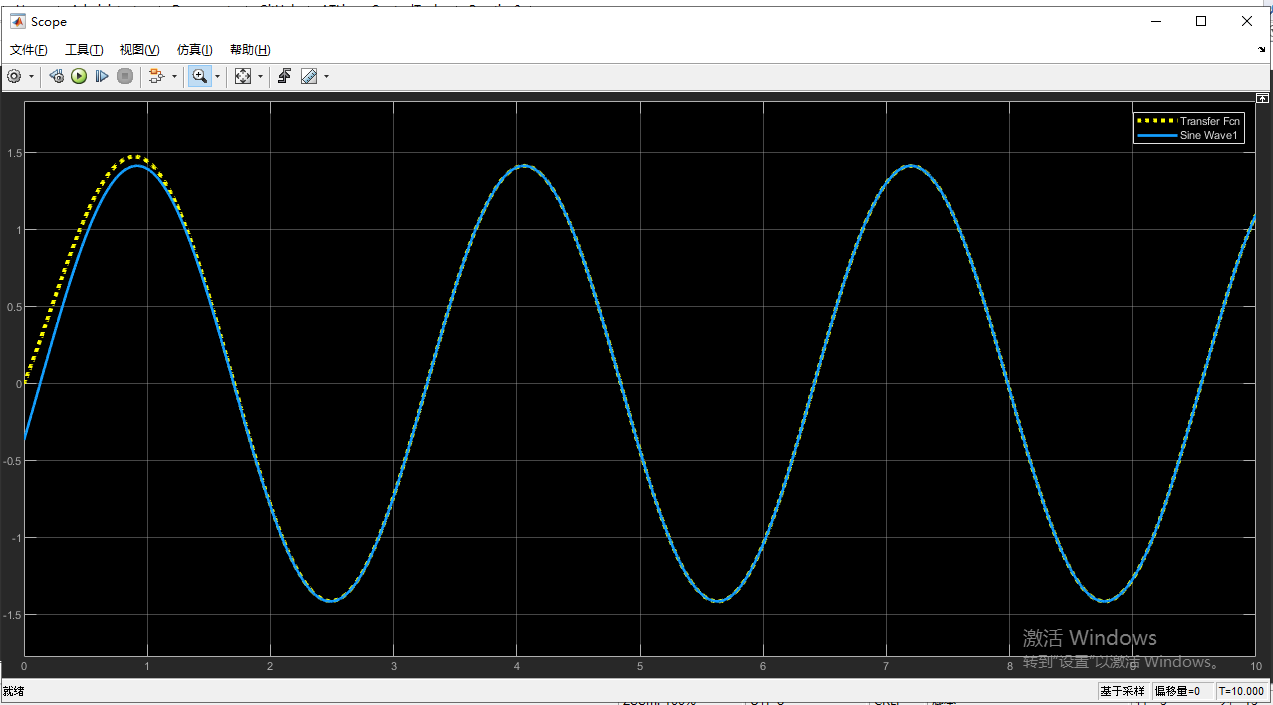
\includegraphics[width = 0.9\linewidth]{Q1Omega_eq2}
                \caption{ $\omega = 2 $}
                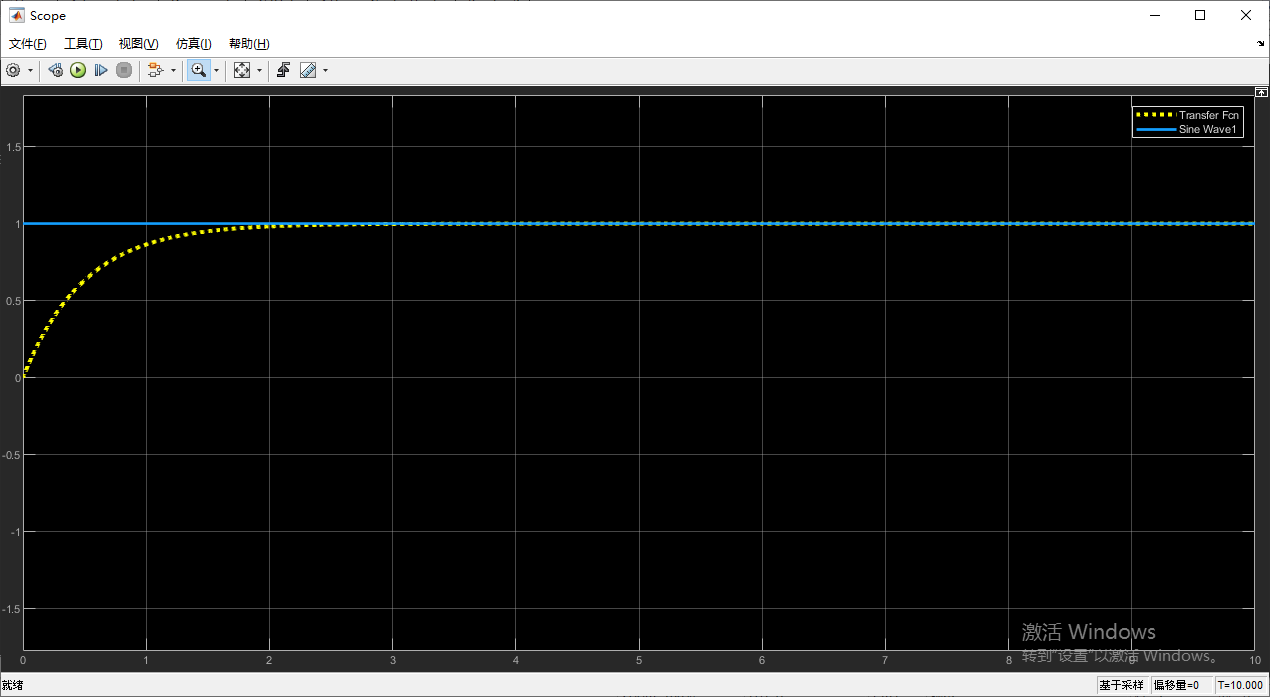
\includegraphics[width = 0.9\linewidth]{Q1Omega_eq0}
                \caption{ $\omega = 0 $}
                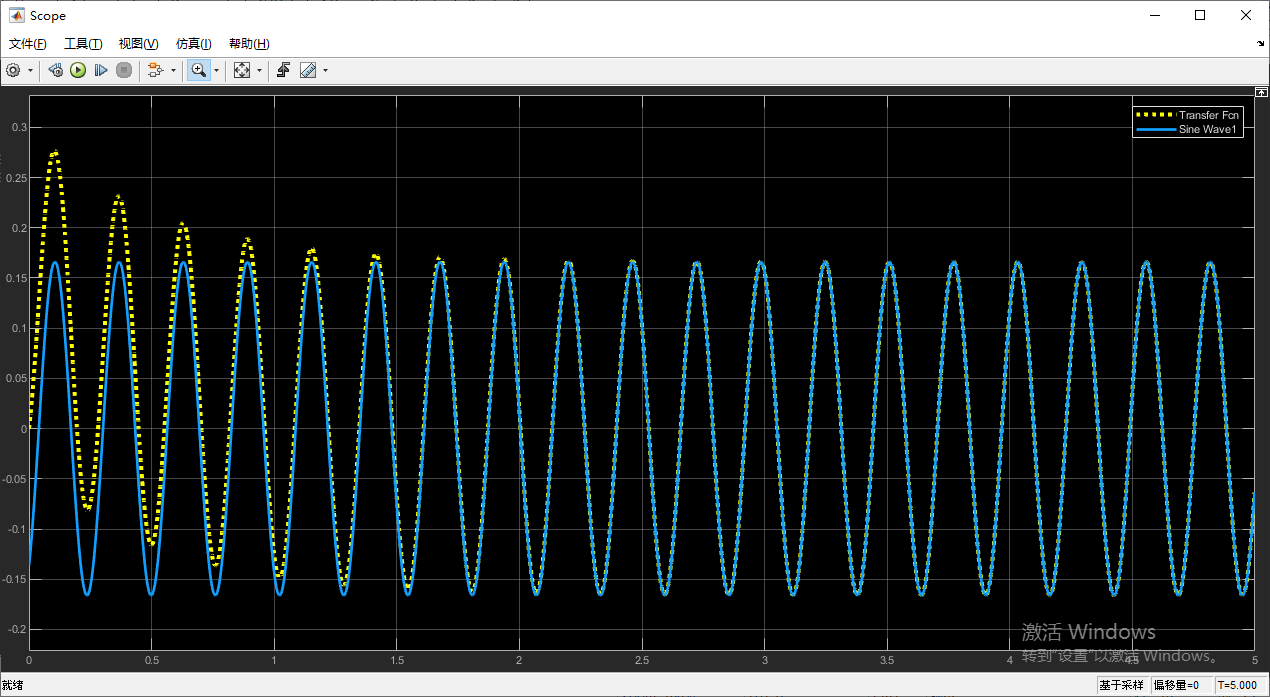
\includegraphics[width = 0.9\linewidth]{Q1Omega_eq3k}
                \caption{ $\omega = 3k $ }
            \end{figure}
    \subsection{Question2}
        \subsubsection{Calculation}
            $$9\ddot{y}(t) + 36\dot{y}(t) + 36y(t) = 4u(t)$$
            Do laplace transform get:
            $$y(s) = \frac{4}{9s^2+36s+36}u(s)$$
            $$W(s) = \frac{4}{9s^2+36s+36}$$
            Let $s = j\omega$.
            $$W(j\omega) = \frac{4}{-9\omega^2+36j\omega+36}$$
            $$W(j\omega) = \frac{4(-9\omega^2+36-36j\omega)}{(36-9\omega^2)^2+(36\omega)^2}$$
            $$P(\omega) = Re(W(j\omega)) = \frac{4(-9\omega^2+36)}{(36-9\omega^2)^2+(36\omega)^2}$$
            $$Q(\omega) = Im(W(j\omega)) = \frac{4(-36\omega)}{(36-9\omega^2)^2+(36\omega)^2}$$
            $$A(\omega) = \sqrt[2]{P(\omega)^2 + Q(\omega)^2} = \frac{4\sqrt[2]{(36-9\omega^2)^2+(36\omega)^2}}{(36-9\omega^2)^2+(36\omega)^2}$$
            $$\phi(\omega) = atan2(Q(\omega),P(\omega))$$
            If $u(t) = Asin(\omega t+\phi_0)+b_0$

            $$y(t) = A(\omega)A_0sin(\omega t + \phi_0 + \phi(\omega)) + b_0$$
        \subsubsection{Graph}
            \begin{figure}[H]
                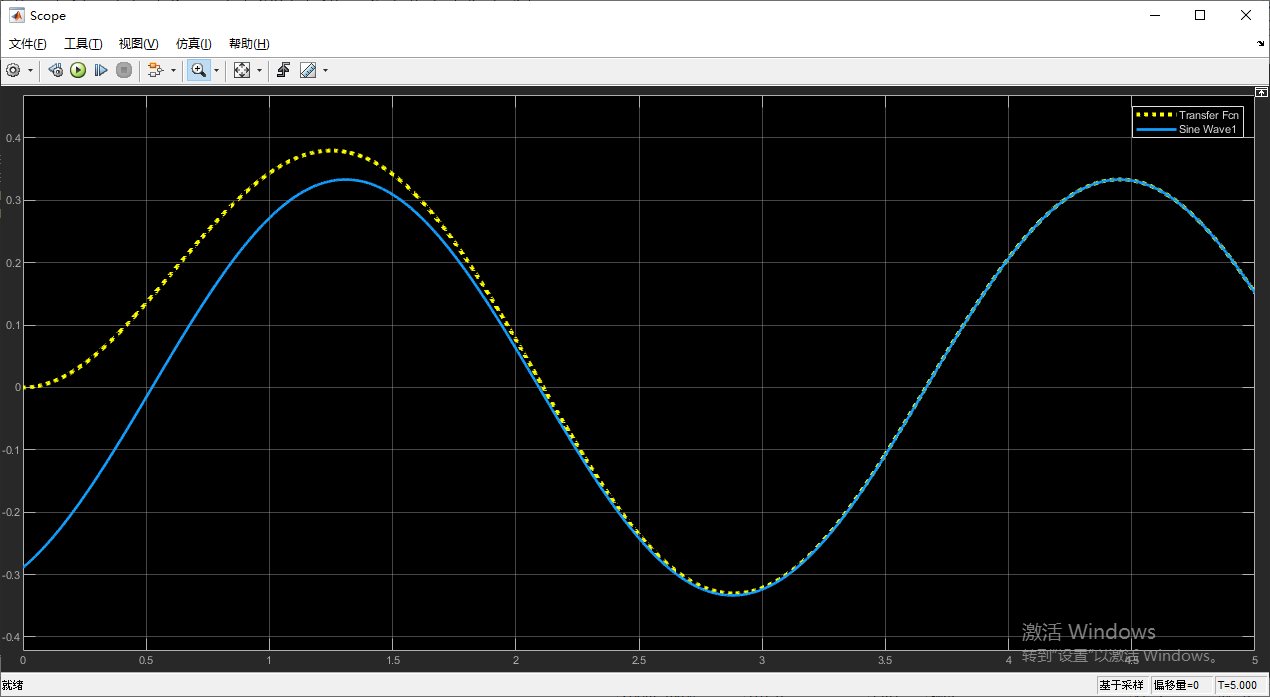
\includegraphics[width = 0.9\linewidth]{Q2Omega_eq2}
                \caption{ $\omega = 2 $}
                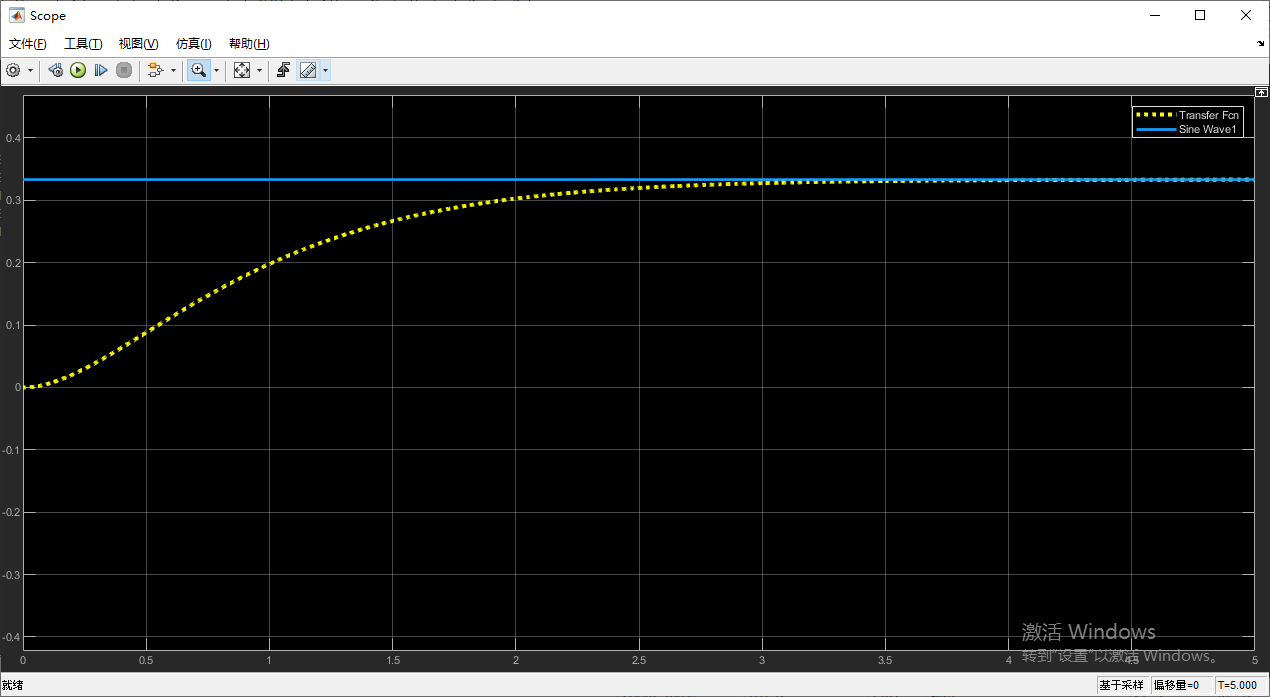
\includegraphics[width = 0.9\linewidth]{Q2Omega_eq0}
                \caption{ $\omega = 0 $}
                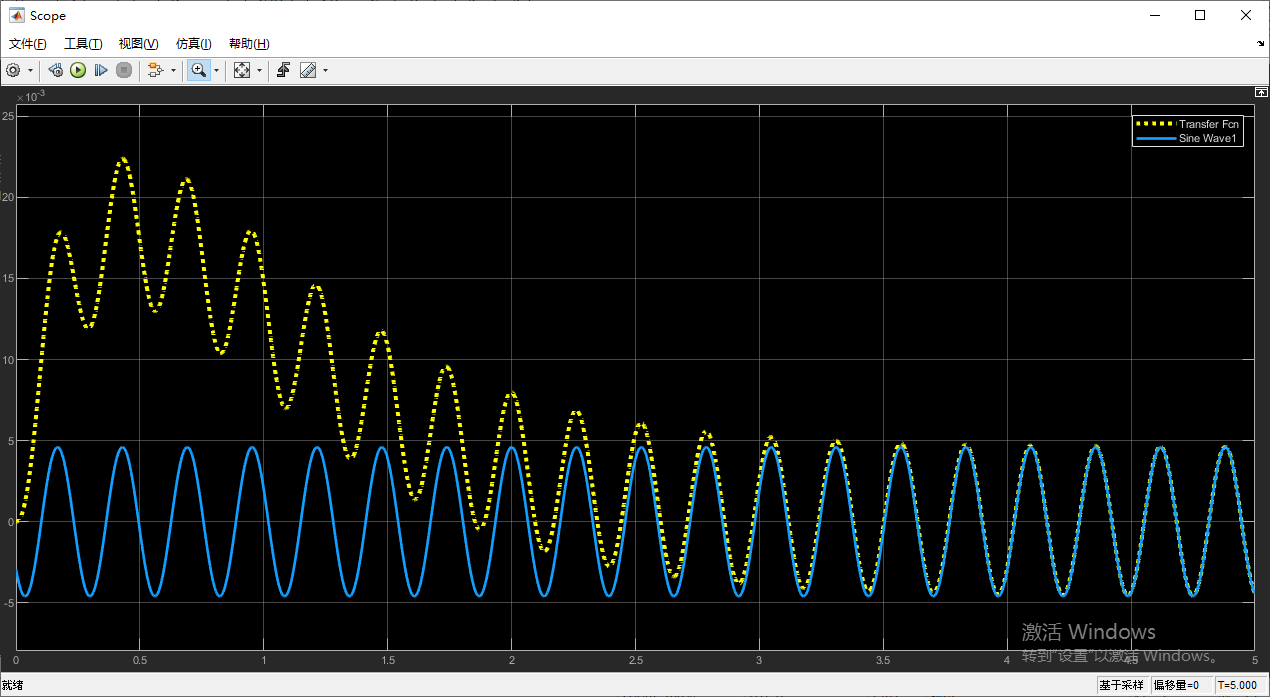
\includegraphics[width = 0.9\linewidth]{Q2Omega_eq3k}
                \caption{ $\omega = 3k $ }
            \end{figure}
    \subsection{Question3}
        \subsubsection{Calculation}
            $$2\ddot{y}(t) + 3\dot{y}(t) + 18y(t) = 18u(t)$$
            Do laplace transform get:
            $$y(s) = \frac{18}{2s^2+3s+18}u(s)$$
            $$W(s) = \frac{18}{2s^2+3s+18}$$
            Let $s = j\omega$.
            $$W(j\omega) = \frac{18}{-2\omega^2+3j\omega+18}$$
            $$W(j\omega) = \frac{18(-2\omega^2+18-3j\omega)}{(18-2\omega^2)^2+(9\omega)^2}$$
            $$P(\omega) = Re(W(j\omega)) = \frac{18(-2\omega^2+18)}{(18-2\omega^2)^2+(9\omega)^2}$$
            $$Q(\omega) = Im(W(j\omega)) = \frac{18(-3\omega)}{(18-2\omega^2)^2+(9\omega)^2}$$
            $$A(\omega) = \sqrt[2]{P(\omega)^2 + Q(\omega)^2} = \frac{18\sqrt[2]{(18-2\omega^2)+(9\omega^2)}}{(18-2\omega^2)^2+(9\omega)^2}$$
            $$\phi(\omega) = atan2(Q(\omega),P(\omega))$$
            $u(t) = Asin(3t+\frac{\pi}{2}+\frac{10k\pi}{180})+k$

            $$y(t) = A(3)sin(3t+\frac{\pi}{2}+\frac{10k\pi}{180}) + k = 2sin(3t+\frac{\pi}{2}+\frac{10k\pi}{180})+k$$
        \subsubsection{Graph}
            \begin{figure}[H]
                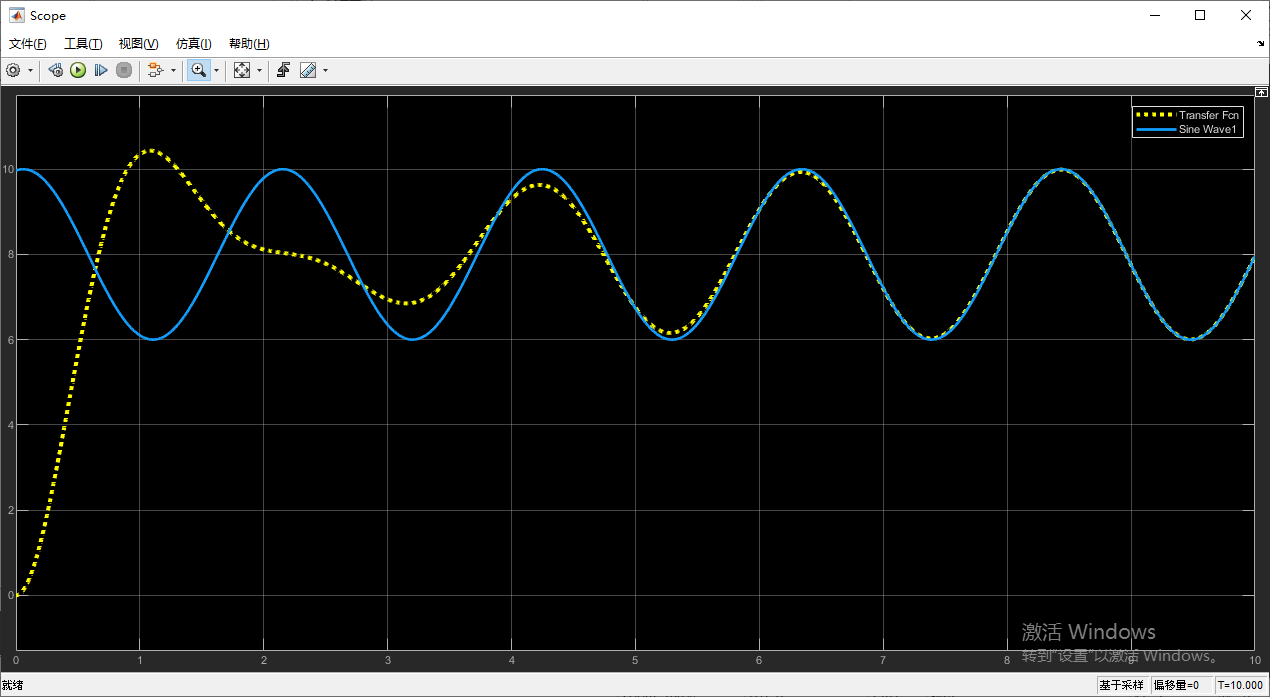
\includegraphics[width = 0.9\linewidth]{Q3}
            \end{figure}
    \subsection{Question4}
        \subsubsection{Failed}
        Reason:

        Let$u(t) = 0$.

        Think about how to solve $2\ddot{y}-3\dot{y}+18=0$.

        And then consider about equation $2\lambda^2-3\lambda+18=0$.
        
        Get that
        $$Re(\lambda) = \frac{3}{4} > 0$$
        Then the system is \textcolor{red}{\textbf{unstable}}.So our method \textbf{Failed}.
        \subsubsection{Graph}
            \begin{figure}[H]
                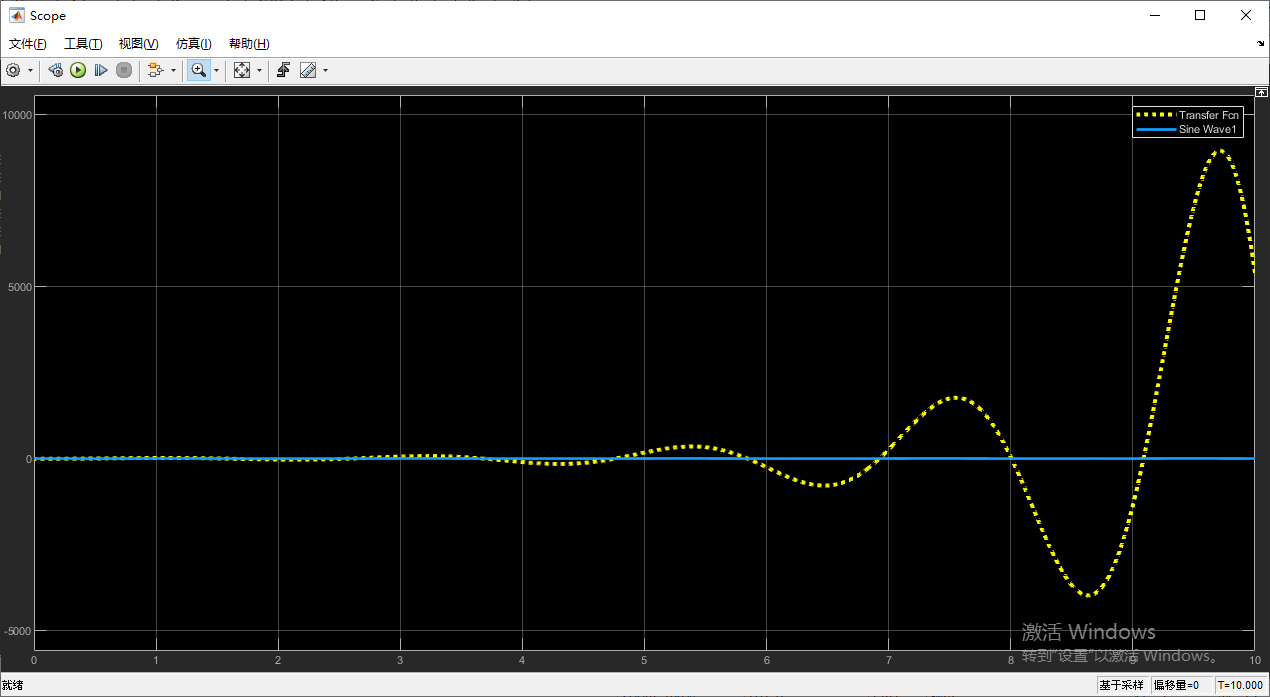
\includegraphics[width = 0.9\linewidth]{Q4Non-stableFails}
            \end{figure}
\end{document}